\section{译者补充:几何光学}\label{sec:译者补充:几何光学}

\begin{remark}
    本节内容不是原书内容,而是译者根据《Optics》\citep{hecht2016optics}
    补充的,请酌情参考和斧正。然而本节仍需要读者对光与波的基本物理概念有所了解,
    这些内容一般可在中学和大学物理教材中找到。
\end{remark}

\subsection{光学背景知识}\label{sub:光学背景知识}
光是人眼可见频段的电磁波,可在真空与介质中传播。
光在真空中的传播速度最大,在介质中的传播速度与介质类型有关。
\begin{definition}
    三维中的\keyindex{波前}{wavefront}{}是某一时刻波\keyindex{相位}{phase}{}相同的点构成的面。
\end{definition}
\begin{definition}
    电磁波在真空中的传播速度$c$与在介质中的传播速度$v$的比值
    定义为\keyindex{绝对折射率}{absolute index of refraction}{index of refraction折射率},
    可简称折射率:
    \begin{align}
        n=\frac{c}{v}\, .
    \end{align}
\end{definition}
\begin{corollary}
    任意介质的绝对折射率都大于1。
\end{corollary}

光传播时在两种介质交界面上会发生\keyindex{反射}{reflection}{}
和\keyindex{折射}{refraction}{},如\reffig{6.26}所示:
其中上层与下层介质的绝对折射率分别为$n_i$和$n_t (n_i<n_t)$;
入射光线、反射光线、折射光线与界面法线的夹角$\theta_i, \theta_r, \theta_t$分别称为
\keyindex{入射角}{angle of incidence}{}、
\keyindex{反射角}{angle of reflection}{}、
\keyindex{折射角}{angle of refraction}{}。
入射光线和界面法线确定的平面称为\keyindex{入射平面}{plane of incidence}{}。
\begin{figure}[htbp]
    \centering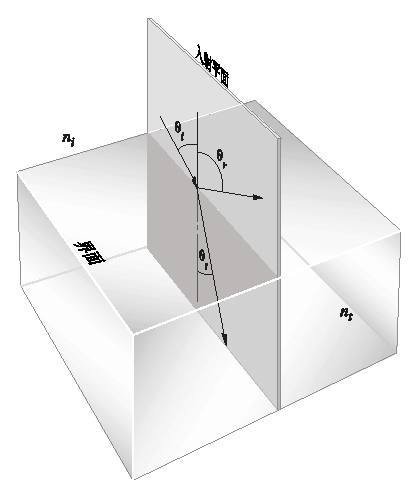
\includegraphics[width=0.5\linewidth]{chap06/ReflectionAndRefraction.eps}
    \caption{反射与折射分别遵循反射定律和折射定律。}
    \label{fig:6.26}
\end{figure}

\begin{proposition}
    \keyindex{反射定律}{law of reflection}{}:反射光线在入射平面内;
    反射光线和入射光线分居界面法线两侧;反射角等于入射角,即
    \begin{align}
        \theta_r=\theta_i \, .
    \end{align}
\end{proposition}
\begin{proposition}
    \keyindex{折射定律}{law of refraction}{}:折射光线在入射平面内;
    折射光线和入射光线分居界面法线两侧;折射角与入射角遵循\keyindex{斯涅尔定律}{Snell's law}{},即
    \begin{align}
        n_i\sin\theta_i=n_t\sin\theta_t \, .
    \end{align}
\end{proposition}
\begin{corollary}
    光线进入更大折射率的介质时会更偏向界面法线,
    进入更小折射率介质时则会更偏离法线。
\end{corollary}
\begin{definition}
    两种介质的绝对折射率之比定义为\keyindex{相对折射率}{relative index of refraction}{index of refraction折射率}:
    \begin{align}
        n_{ti}=\frac{n_t}{n_i}\, .
    \end{align}
    由此斯涅尔定律也可写作:
    \begin{align}
        \frac{sin\theta_i}{\sin\theta_t}=n_{ti}\, .
    \end{align}
\end{definition}

我们考虑\reffig{6.27}的情景:一束光线从点$S$起依次穿过$m$层介质并发生折射,
最终到达点$P$。设在每种介质中传播时对应的介质绝对折射率、路程、传播速度
分别为$n_j, s_j, v_j (j=1,\ldots,m)$。于是光线传播的总时间为
\begin{align}
    t=\sum\limits_{j=1}^{m}{\frac{s_j}{v_j}}\, ,
\end{align}
利用绝对折射率的定义可得
\begin{align}
    t=\frac{1}{c}\sum\limits_{j=1}^{m}{n_js_j}\, .
\end{align}
相对于空间路程$\sum\limits_{j=1}^{m}{s_j}$,
我们定义上式中的$\sum\limits_{j=1}^{m}{n_js_j}$
为\keyindex{光程}{optical path length}{}(OPL)。
更一般地,在非均匀介质中折射率是位置的函数,因此有
\begin{align}
    OPL=\int_S^P {n(s)\mathrm{d}s}\, .
\end{align}
\begin{figure}[htbp]
    \centering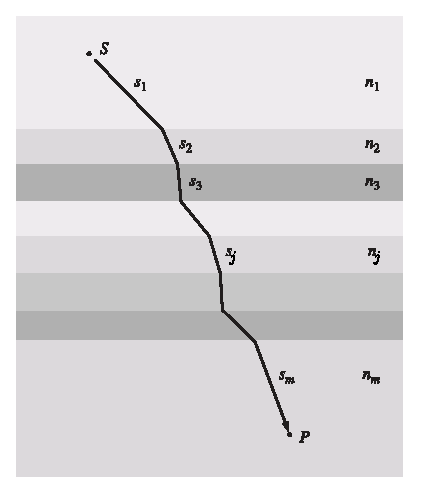
\includegraphics[width=0.5\linewidth]{chap06/PropagatingThroughLayeredMaterial.eps}
    \caption{在多层介质中传播的光线。}
    \label{fig:6.27}
\end{figure}

事实上,包括反射与折射在内,光的一般传播规律遵循费马原理。
它可推导出光线在真空中沿直线传播的性质以及反射定律和折射定律。
\begin{proposition}
    \keyindex{费马原理}{Fermat's principle}{}的现代形式是:
    光线从点$S$到点$P$的传播路径一定是对光程\keyindex{稳定}{stationary}{}的。
\end{proposition}

\begin{figure}[htbp]
    \centering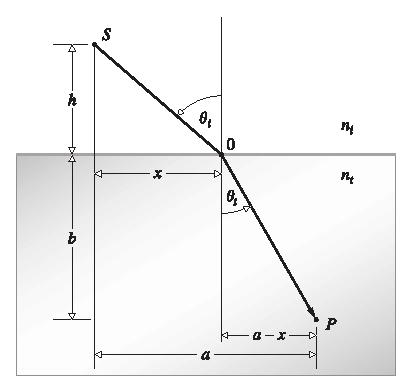
\includegraphics[width=0.5\linewidth]{chap06/FermatsPrincipleAppliedToRefraction.eps}
    \caption{费马原理运用于折射。}
    \label{fig:6.28}
\end{figure}

如\reffig{6.28}所示,我们利用费马原理来推导斯涅尔定律:
\begin{prove}
    考虑从点$S$到点$P$的光线,它在界面上点$O$处发生折射,
    相应量已标在途中图中。其光程为
    \begin{align}
        OPL=n_i\overline{SO}+n_t\overline{OP}=n_i\sqrt{x^2+h^2}+n_t\sqrt{b^2+(a-x)^2}\, .
    \end{align}

    依据费马原理,我们令$\displaystyle\frac{\mathrm{d}OPL}{\mathrm{d}x}=0$,可得
    \begin{align}
        \frac{n_ix}{\sqrt{x^2+h^2}}-\frac{n_t(a-x)}{\sqrt{b^2+(a-x)^2}}=0\, .
    \end{align}
    注意到$\displaystyle\sin\theta_i=\frac{x}{\sqrt{x^2+h^2}}$以及
    $\displaystyle\sin\theta_t=\frac{(a-x)}{\sqrt{b^2+(a-x)^2}}$,带入得
    \begin{align}
        n_i\sin\theta_i=n_t\sin\theta_t\, .
    \end{align}
    即得到斯涅尔定律。
\end{prove}

自身发光或被照亮的物体可以视作是大量辐射点\keyindex{源}{source}{}构成的。
每个点源都在发出\keyindex{球面波}{spherical wave}{}。
此时我们说光线从给定点源\keyindex{发散}{diverge}{}。
反之,若球面波坍缩到一点,我们说光线\keyindex{汇聚}{converge}{}到该点。
实际中我们往往只处理\keyindex{波前}{wavefront}{}的一部分。